\documentclass{article}
\usepackage{filecontents}
\usepackage[left=2.5cm,top=2.5cm,right=2.5cm,bottom=2.5cm]{geometry}
\usepackage{amsmath}
\usepackage{array}
\usepackage{caption}
\usepackage{longtable}
\usepackage{placeins}
\usepackage{graphicx}
\usepackage{subcaption}
\usepackage{setspace}
\usepackage{animate}
%\usepackage[active,tightpage]{preview}
\usepackage{natbib}
\bibpunct{(}{)}{,}{a}{}{;} 
\usepackage{url}
\usepackage{nth}
\usepackage{authblk}
\usepackage{listings}
% for the d in integrals
\newcommand{\dd}{\; \mathrm{d}}
\newcommand{\tc}{\quad\quad\text{,}}
\newcommand{\tp}{\quad\quad\text{.}}
\newcommand{\un}[1]{\underline{#1}}
\bibliographystyle{apalike}

\title{Deviations in avoidable causes of death in adulthood drive mortality
inquality between Mexican states}

%\author[1]{Nancy Plascencia\thanks{nancy.plascemcia@agricomer.com}}
\author[1,2]{Jose Manuel Aburto}
%\author[3]{Ainhoa Alustiza}
\author[2]{Tim Riffe}
\affil[1]{European Doctoral School of Demography}
\affil[2]{Max Planck Institute for Demographic Research}


\begin{document}

\maketitle

\begin{abstract}
We analyze trends in temporary life expectancy for three large age groups from
1990 to 2015 for all 32 Mexican states, and compare these with a low
mortality benchmark. We assess the impact of avoidable/amenable mortality on
temporary life expectancy at the state level by sex. We apply demographic
measures and use standard decomposition techniques to disentangle the impacts
of selected causes of death on trends in state health inequality.
We find improvements in temporary life expectancy for the population aged 0 to
14, as they continuously approached the low mortality benchmark. However, the
adult population aged 15 to 39 shows deterioration among males after 2006 in
almost every state. Females on the whole converged toward the low mortality
benchmark in the same age group. Adults aged 40 to 74 show an unexpected
decrease in the low mortality benchmark, indicating universal deterioration in
temporary life expectancy for thsi age group, albeit with wide variation
between states. These findings support the case for reforms that treat all
causes of death as public health priorities, and that target regional
disparities in health.
​\end{abstract}

\section*{Key messages}
\begin{itemize}
\item Reducing health inequalities among sub-populations is a goal of every
developing country. Addressing such inequalities in adult populations in
Mexico is proving to be a challenge to reaching this goal.
\item We hypothesize age-dependent variations in temporary life expectancy
between states, particularly due to the rise in homicide mortality and the
increase of conditions amenable to medical services and policy/behavior actions.
\item Our results show that deviations from our low mortality benchmark are
mainly driven by adult mortality. Young-age mortality has steadily converged
toward the low mortality benchmark, pointing towards the success of public
health interventions.
\item Cirrhosis, homicide, diabetes and isquemic heart diseases contribute the
most to the persistence of health inequalities between Mexican states.
Importantly, some states could gain up to two years of life on average if the
low mortality benchmark were acheived.
\end{itemize}

\begin{spacing}{1.5}
\section*{Introduction (max 6000 words)}
The \nth{20} century was marked by sizable improvements in mortality, living
conditions and health in most Latin American countries \citep{who2000}. 
In Mexico, these improvements have slowed down recently as a result of opposing
trends in particular causes of death. For instance, homicide and diabetes
increased dramatically, even as infectious and
respiratory diseases continued to fall. While life
expectancy at birth increased by 4.3 years for males (from 67.6 to 71.9) and 3.4
for females (from 73.8 to 77.2) between 1990 and 2000 \citep{SOMEDE},
between 2000 and 2010, life expectancy at birth entered into a period of
stagnation for males and slowed progress for females \citep{canudas2014}. 

% TR: give program rollout dates because people will want to compare them with 
% the trend lines.
\un{This
period} coincides with the implementation of different public health
interventions, such as the Universal Vaccination Program and Seguro
Popular, which aim to provide primary and secondary
health care to the uninsured population and allocate funds to cover catastrophic
health expenditures \citep{knaul2005}. Further, the Oportunidades program
was introduced to supply incentives for families to invest in themselves and
benefit from education, health, and nutrition in the late 1990's \citep{neufeld2012}. Some evidence
suggests that Mexico experienced substantial decreases in infant and child
mortality, along with improvements that contributed to the reduction of
mortality and in the prevalence of acute malnutrition between 1980 and 2000
because of these interventions \citep{sepulveda2006}. Similarly, some evidence
suggests that by 2012 Seguro Popular had covered an additional 52 million
people in Mexico that did not have any access to public health care and, as a result, there has been a reduction in catastrophic health expenditures \citep{knaul2012}.

 These results underscore the progress in public health interventions, but they
 do not reveal heterogeneity between Mexican states or the epidemiological patterns
 of different age groups. Given improvements in health care coverage, the strong
 role of institutions, and ongoing public health interventions, it is necessary to assess the varied
 impacts that these interventions may have had on mortality in Mexican
 states. For instance, Oportunidades is focused on the poorest
 states, and Seguro Popular was introduced at different times in different
 states \citep{Frenk2006}. It is therefore important to describe the high degree
 of social and health inequalities in Mexico. The age dimension of
 mortality inequality is important in part due to anticipated population ageing
 in the coming decades. For example, the percentage of the population aged 60 or
 older increase from 10\% in 2015 to 15\% in 2030 \citep{CONAPO}.
 
% Moreover, it is important to identify potential opportunities to improve and
 % put forward solutions to reduce the gap of the unequal impact of public health interventions caused by the heterogeneity in how these interventions have taken place within the states.
 
 
 % TR: on average, by 17\%  for males and 14\% for females ---- per annum or
 % total?
 One approach to assess the impact of health services is by operationalizing the
 concept of Avoidable/Amenable Mortality (hereafter abbreviated AM)
 \citep{nolte&mckee2004, nolte&mckee2008}. This construct aims to measure the quality of health service systems by selecting certain
 causes of death that should not occur in the presence of effective and
 timely health care. Among industrialized countries (e.g., United States,
 Australia, France, Japan), a reduction in AM rates was
 observed from the late 1990's into the \nth{21} Century
 \citep{nolte&mckee2008}. Avoidable mortality rates fell, on average, by 17\%
 for males and 14\% for females in these countries. Despite mortality reductions for
 both sexes, heterogeneity between countries persists, with the United
 States showing the smallest reductions (around 5\%) for both sexes. However,
 each country showed progress in mortality from treatable cancers and
 circulatory diseases except for ischemic heart diseases.

In Mexico, the components of avoidable mortality had different trends since the
late 1990's. Between 2000 and 2004 AM decreased, particularly from
infectious diseases and nutrition-related conditions \citep{francomarina2006}, while it increased between 1998 and 2010 due to diabetes, circulatory diseases, perinatal and respiratory conditions
\citep{agudelo2014efecto}. Increases in the latter causes
of death were particularly concentrated in the poorest states of the country
\citep{davila2014mortalidad}. We aim to extend these studies
by a more focused segmentation of AM into health intervention-related AM and
behavior-related AM. Also, we extend analysis to all 32 states, by sex, and over
the full 26-year period from 1990 to 2015. Finally, we compare state mortality patterns
with an easy-to-understand low-mortality benchmark calculated for large age
groups (e.g., 0-14, 15-39, 40-75).
This low-mortality benchmark is calculated on the basis of the lowest observed
mortality rates within ages and causes, selected from the full set of 32 Mexican
states.
This concept was first proposed by \citet{whelpton1947}, and later explored by 
\citet{wunsch1975minimum} and \citet{vallin2008minimum}. Deviations from the
low-mortality benchmark indicate a strong potential for improvement. We apply
demographic measures and standard decomposition techniques to isolate the cause
and age-specific deviations between states and the corresponding optimal
lifetable.

We hypothesize age-dependent variations in temporary life expectancy outcomes.
In particular, we expect convergence between states in temporary life expectancy
for young people, since public health interventions are mainly focused in infant
mortality and child health. For instance, the vaccination program and the health
reform aim to provide universal coverage to children in Mexico. Recent
evidence suggests a decrease in mortality between ages 0 to 14 due to a decline
in infectious and respiratory diseases \citep{canudas2014}. On the contrary, we
expect little improvement in temporary life expectancy for the adult and older
adult population, due to the unprecedented rise in homicide mortality and the
increase in diabetes mortality along with endocrine/metabolic diseases \citep{canudas2014}. Although every
state has the commitment to providing universal coverage and equitable access to
health care since the early 2000's, we anticipate heterogeneity between states
in mortality improvements due to state differences in epidemiological patterns
and differences in how benefits of health care programs have been delivered to
the population \citep{Frenk2006}.


\section*{Data \& Methods} 
Our analyses are based on publicly available anonymized datasets.%
% Therefore, ethical approval for human subject research from the Institutional Review Board of the respective institutions was exempted.
We used deaths microdata available from official files produced by
the Mexican Statistical Office from 1990 to 2015 \citep{INEGI}. These data
contain necessary information on causes of death by single age, sex, and state
of residence at the time of death. Population estimates from 1990 to
2010 came from the Mexican Society of Demography \citep{SOMEDE}. These
estimates adjust for age misstatement, undercounting, and interstate
and international migration. Additionally, we estimate intercensal population
counts by age, sex and state for the period 2011-2014 using the most recent
inter-census survey that took place in 2015 \citep{INEGI}. Death counts and
population exposures were used to calculate cause-age-specific death rates by
sex and state from 1990 to 2014 \citep{SOMEDE}.

\subsection*{Classification of Causes of Death}
% TR: intersectoral??
To separate causes of death that are susceptible to medical intervention (e.g.,
infectious and respiratory diseases) and those related to health behaviors and
intersectoral policies (e.g., homicides, lung cancer) we use the concept of
'Avoidable/Amenable Mortality' (AM) \citep{nolte&mckee2004, nolte&mckee2008}. This
concept assumes a list of conditions that should not cause death if timely
medical care is available. Recently, this concept has also been used to gauge
the effect of causes that can be influenced by public policy (e.g., cirrhosis) \citep{elo2014}. We classified causes of death into ten groups based on prior studies \citep{elo2014, Aburto2015}, as listed in Table~\ref{tab:causes}, with
relative frequencies by sex.

% latex table generated in R 3.1.2 by xtable 1.7-4 package
% Wed Sep 23 21:57:18 2015
\begin{table}[ht]
\centering
\caption{Avoidable Mortality classification, with crude percentages below age 75.}
\label{tab:causes}
\begin{tabular}{>{\raggedright}m{3cm}rr}
Group/Cause  & Males & Females \\ 
  \hline
Causes amenable to medical service & 28.50 & 40.24 \\ 
  Diabetes & 9.07 & 14.77 \\ 
  Ischemic heart diseases & 7.92 & 6.66 \\ 
  HIV/AIDS & 1.80 & 0.51 \\ 
  Lung cancer & 1.58 & 1.09 \\ 
  Cirrhosis & 5.34 & 1.09 \\ 
  Homicide & 5.95 & 1.05 \\ 
  Road traffic accidents & 5.82 & 2.26 \\ 
  Suicide & 1.48 & 0.46 \\ 
  Other causes & 32.53 & 31.86 \\ 
   \hline
\end{tabular}
\end{table}

We separate diabetes, ischemic heart diseases (IHD), HIV/AIDS, lung
cancer, and cirrhosis because all of them are amenable to both health behavior
and medical service, and because the first two represent major causes of death
in Mexico \citep{canudas2014}. In addition to these causes, we also separate
homicide, road traffic accidents, and suicide because they have emerged as
leading causes of death among young people, and the first two had a sizeable
impact on life expectancy recently in Mexico \citep{canudas2014}. All causes of
death were classified using the International Classification of Diseases,
revision 9 for the period 1990-1997 and the tenth revision for 1998-2015 (see
Appendix Table 1 for details on ICD codes for each cause). % cite ICD9 and 10,
% unless already cited in appendix

We truncate analysis at age 75 because classification of causes of deaths and
age reporting are considered to be innacurate in death registration at older
ages \citep{tobias2001}. Most changes in life expectancy are
likely due to changes in mortality patterns below the age of 75 \citep{Aburto2015}. In addition, health care and policy/behavior interventions are more likely to be effective at younger ages \cite{elo2014}.


\subsection*{Demographic Methods}
We smooth cause-specific death rates over age and time for each
state and sex separately using the 2-d p-spline method proposed by
\citet{GC2012}.
This helps eliminate stochastic zeros, which otherwise would accumulate in the
minimum mortality schedule. Smoothed death rates are then constrained to sum to
the unsmoothed all-cause death rates. We then calculate period life tables up to age 74 for males and females from 1990 to 2014 following the HMD Methods
Protocol \citep{HMDMP}. We calculate temporary life expectancy to
capture differential effects of mortality in three large age
groups: children (ages 0-14), young adults (ages 15-40) and older adults
(40-74). %We do this following the formulas of \citet{arriaga1984}, as
%defined below.

We estimate cause-specific contributions to the difference between
state-specific temporary life expectancy and benchmark temporary life expectancy
($e^{\star}$) applying standard decomposition methods
\citep{horiuchi2008}. Decomposition techniques are a suitable method for comparing life expectancies across populations and analyzing age and cause-specific contributions to their differences \citep{preston2001}. All the analyses were carried out
using \texttt{R}.

\subsection*{Low-mortality benchmark}
This approach was first proposed by \citet{whelpton1947}, and we summarize it
briefly here. The low-mortality lifetable is based on synthetic mortality
rates, defined as the sum of the lowest observed mortality rates by age, cause,
from among all states for a given sex and year. %In continuous terms, we define
% life expectancy, $e(0)$, as:
%\begin{equation}
%\int _0 ^\infty \ell(x) \dd x \tc
%\end{equation}
%where $\ell(x)$ is the survivorship function defined with radix of one%, or as
% a function of the force of mortality, $\mu(x)$ as:
%\begin{equation}
%\label{eq:lx}
%\ell(x) = e^{-\int_0^x \mu(a) \dd a}
%\end{equation}
The low mortality rates, $\mu(x)^{\star}$, are calculated as the sum of $C$
cause-specific minimum mortality rates at age $x$, under the assumption that
causes of death are independent of one another:
\begin{equation}
\label{eq:mxmin}
\mu(x)^{\star} = \sum_{c=1}^C min(\mu(x,c,s)) \tc
\end{equation}
where $x$ is age, $c$ is the given cause, and $s$ indexes the set of 32 states
from which the minimum is selected. The resulting minimum mortality rate schedule
($\mu^{\star}(x)$) has a unique age profile, and it determines our benchmark life expectancy, $e(0)^{\star}$.
$e(0)^{\star}$ can be treated as the maximum presently achievable life
expectancy assuming perfect diffusion of the best available practices and
technologies within a given set of populations \citep{vallin2008minimum}. It is
an imaginary quantity because no particular population is expected to achieve
this mortality pattern. However, this value is a practical reference because it
is based neither on a projection of improvements into the future nor on an
arbitrary and likely dissimilar population. We refer to the state with the
highest life expectancy in a given year as the vanguard state.

\subsection*{Temporary Life Expectancy}

Temporary life expectancy between ages
$x_1$ and $x_2$, for $x_1<x_2$, is defined as the average years of life lived
between these ages according to a given set of mortality rates
\citep{arriaga1984}. We denote this quantity as $e(x_1,x_2)$, and its benchmark
maximum as $e^{\star}(x_1,x_2)$. Defined in terms of lifetable survivorship, $\ell(x)$:

\begin{equation}
e(x_1,x_2) = \frac{\int _{x_1}^{x_2} \ell(x) \dd x}{\ell(x_1)} \tp
\end{equation}

The interpretation of temporary life expectancy has the advantage, that if nobody dies between the starting and ending age, then the maximum life expectancy is $x_2-x_1$.  For example, if we set $x_1=0$ and $x_2=14$, if no person dies between the ages 0 and 14, on average the population lives 14 full years, which means that the temporary life expectancy between these ages, $e(0,14)$, is fourteen. Which sets a maximum achievable and, therefore, measurable.

\subsection*{Limitations}
The limitations of our study should be mentioned. First, mortality data are
likely to present inaccuracies in cause-of-death classification due to
comorbidities, particularly at older ages \citep{tobias2001}. To mitigate this,
we focus on ages below 75, grouping causes of death using ICD codes according to
the avoidable mortality concept.
Second, our estimates regarding homicide mortality are likely to be
underestimated because of inaccurate practices regarding counting, reporting,
and due to the large number of missing individuals in Mexico \citep{HRW2011}.
Third, avoidable mortality should be understood as an indicator of potential
weaknesses with respect to health care and some public health policies and not
as a definitive assessment \citep{nolte&mckee2008}. Fourth, the amount of deaths
that should be considered avoidable within the avoidable classification is not
clear \citep{beltran2011avoidable}. For instance, \citet{nolte2012amenable}
consider only 50 percent of heart disease amenable in industrialized countries,
based on a previous review of evidence.

We do not have information to precisely
measure percentages of avoidable mortality within cause groups. Nonetheless, the
difference between a given mortality schedule and the best practices schedule of
the same year can be conceived of as a minimal definition of avoidable
mortality, a sort of lower bound to how much mortality could have been avoided.
Certainly, even a best practices schedule will contain elements of mortality
most would consider avoidable. To the extent that the components of the BP schedule were indeed
attained somewhere in the population universe, one can view any excess mortality
with respect to the BP schedule as avoidable. Little progress has been made in advancing the concept of avoidable mortality \citep{holland2003}. We believe this perspective improves on the original concept and gauge better the avoidable deaths.

\section*{Results}
\subsection*{Trends in best practices life expectancy}

Figure 1 shows state-specific  (black lines), vanguard  (red lines) and BP (blue lines) remaining life expectancies for ages 0-14 (\ref{fig:e0_14} ), 15-39
(\ref{fig:e15_39}) and 40-74 (\ref{fig:e40_74}). The red line represents the
vanguard life expectancy out of the 32 states within each year and the blue line
represents the maximum potentially achievable for the Mexican population under
the best practices definition.
The figures clearly shows a convergence pattern among the states toward the BP
expectancy through at least the year 2000; however the latter period shows
stagnation and even decreases for some states. Particularly, improvements and a trend to achieve BP is seen between ages 0 and 14. Opposing this trend, male temporary life expectancy between 15 and 39 years shows a clear downward after 2005, with some states experiencing a dramatic deterioration in temporary life expectancy. Results for females show stagnation in achieving BP temporary life expectancy. As in males' results, some states experienced losses of life after 2005, leading to widening the gap between states and BP line. 
Importantly, temporary life expectancy for adults between 40 and 75 years shows stagnation and deterioration during the 20-year period. Even the BP life expectancy exhibits a downward trend, pointing to increases in adult mortality. Furthermore, also the BP line has been moving further from the maximum temporary life expectancy, which means that the survival in this population group is not following the rectangularization hypothesis \citep{wilmoth1999}. 


\begin{figure}
\label{Fig_temporary_le}
\centering
\caption{Temporary life expectancy for states (black line), vanguard life
expectancy (red) and best practices life expectancy by sex, 1990-2015.}
\begin{subfigure}{\textwidth}
\centering
\caption{$e(0,14)$}
\vspace{-2em}
\label{fig:e0_14}
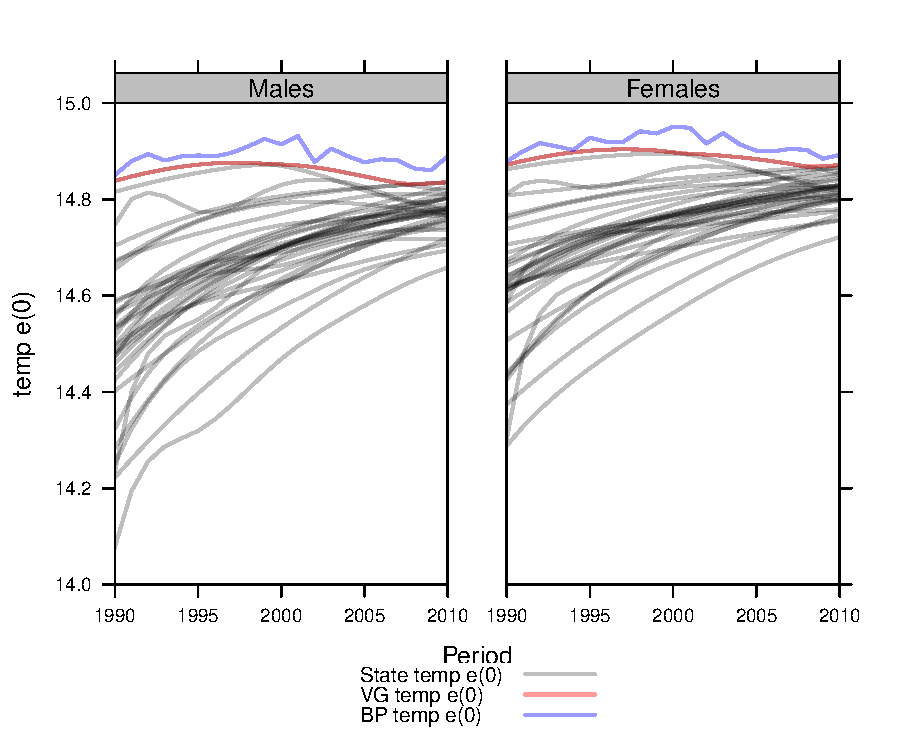
\includegraphics[scale=.5]{Figures/et0_14s.pdf}
\end{subfigure}
\\
\begin{subfigure}{\textwidth}
\centering
\caption{$e(15,39)$}
\vspace{-2em}
\label{fig:e15_39}
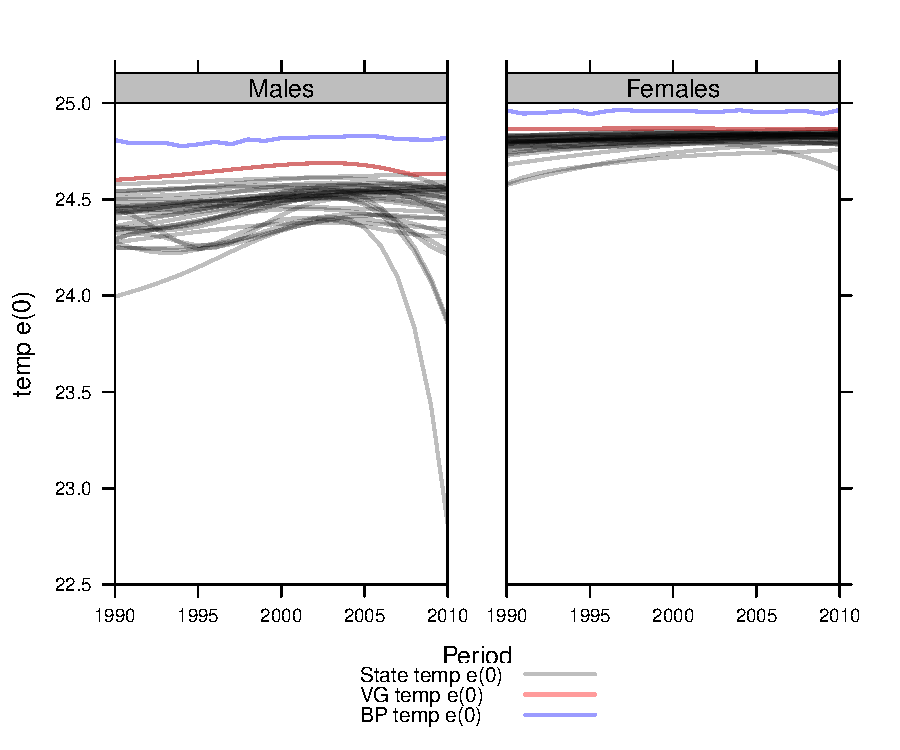
\includegraphics[scale=.5]{Figures/et15_39s.pdf}
\end{subfigure}
\\
\begin{subfigure}{\textwidth}
\centering
\caption{$e(40,74)$}
\vspace{-2em}
\label{fig:e40_74}
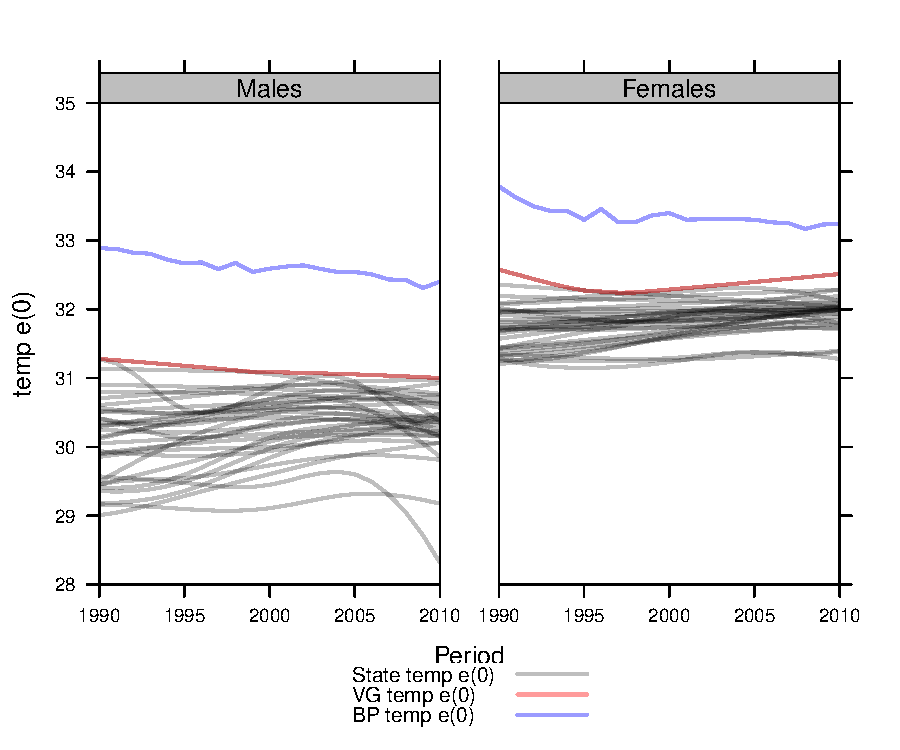
\includegraphics[scale=.5]{Figures/et40_74s.pdf}
\end{subfigure}
Source: own calculations based on INEGI and SOMEDE files. 
\end{figure}

%\FloatBarrier
%\subsection*{State trends in departures from best practices temp e(0)}
%Small multiples maps (time series of maps)


\subsection*{Age and cause-specific contributions to state differences from the best
practices trend. \footnote{This section will be completed at a later date and updated to 2015. Preliminary results are shown.
}}

Figure 2, 3 and 4  show cause-specific contributions of avoidable mortality to the gap between temporary life expectancy and the BP life expectancy for males (panels (a))  and females (panels (b)) between 0 and 14, 15 and 39, and 40 and 74 years respectively. Results near 0 mean that they are very close to the minimum observed among all the states, results greater than zero mean deterioration in mortality relative to the minimum observed. 

Reductions in the gap between the observed life expectancy and the best practices between 0 and 14 years are mainly driven by the causes amenable to medical service (\ref{fig:e0_14_males}). Since the 1990's, reductions in mortality of these articular conditions had led to convergence among the states and reducing health disparities. In some states, the gap went from half a year to less than a quarter of year. The results are similar for men and women (\ref{fig:e0_14_females}). Contributions of the other avoidable categories are negligible. 

Among the young-adult population (15-39), the deviation of the states from BP life expectancy is, almost entirely, explained by homicide mortality and road traffic accidents for males (\ref{fig:e15_39_males}). In the 1990's, some states were more than a quarter of year far from the BP line. This trend was reversed as the 1990's ended and the 2000's begun, almost all the states were less than 0.05 years (blue line) from achieving the minimum homicide-mortality observed in the country. Nevertheless, after 2005, an upward trend is documented, with some states experiencing deviations from the best practices over half a year (first red line). Similar trends are observed in women (\ref{fig:15_39_females}) but with lower magnitude. The impact of the rest of AM categories is negligible. 


\begin{figure}
\label{fig:0-14_contributions}
\centering
\caption{Age and cause contributions to state differences from the best
practices trend for temporary life expectancy 0-14, 1990-2015.}
\begin{subfigure}{\textwidth}
\centering
\caption{Males}
\vspace{-2em}
\label{fig:e0_14_males}
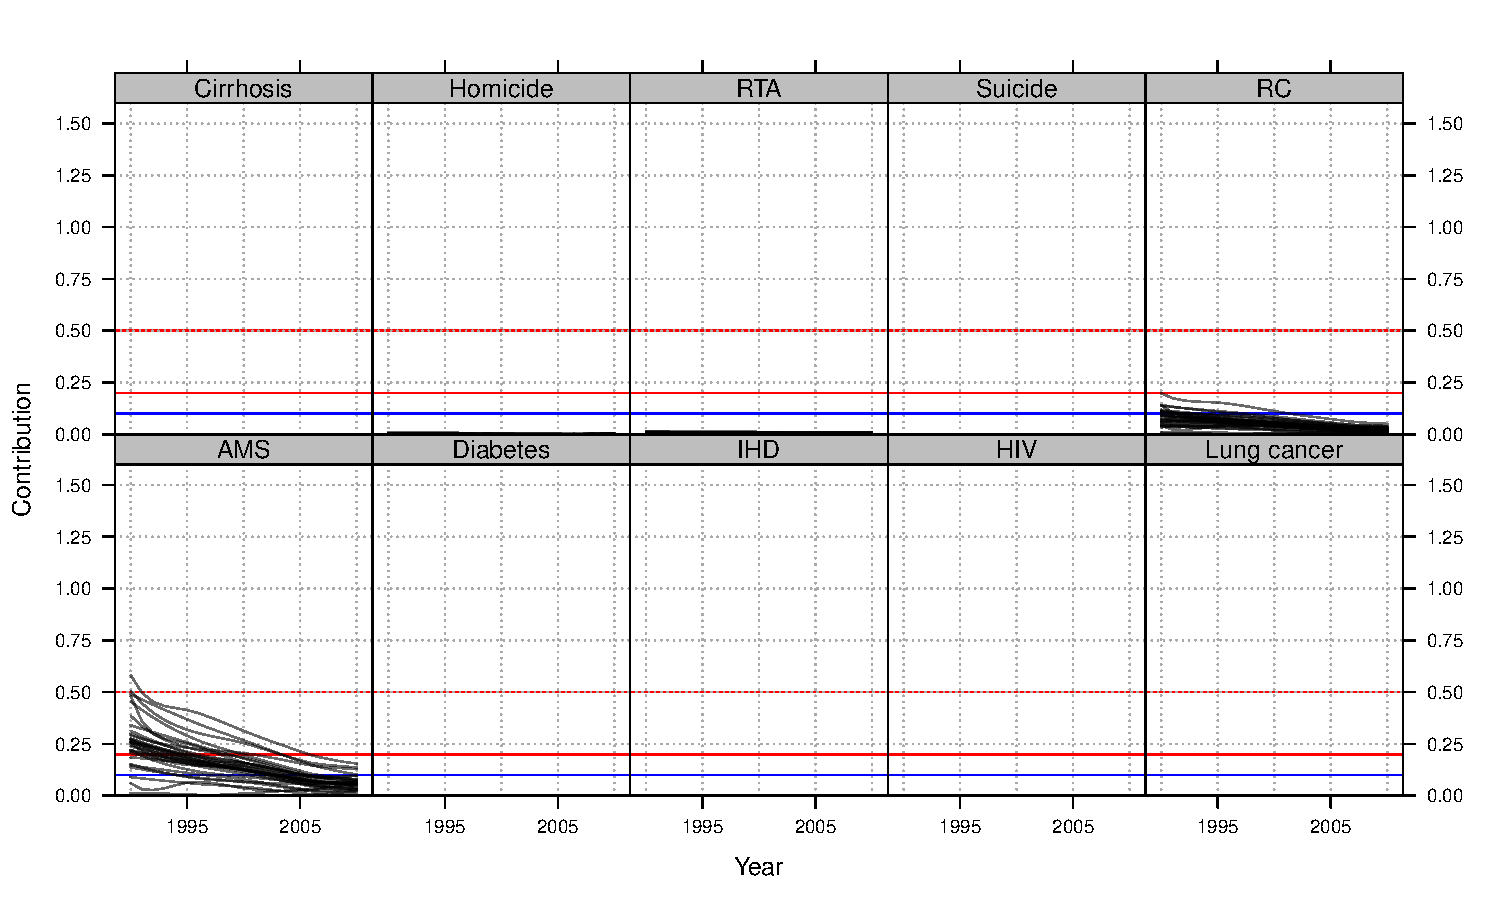
\includegraphics[scale=.5]{Figures/AM_0_14_males.pdf}
\end{subfigure}
\\
\begin{subfigure}{\textwidth}
\centering
\caption{Females}
\vspace{-2em}
\label{fig:e0_14_females}
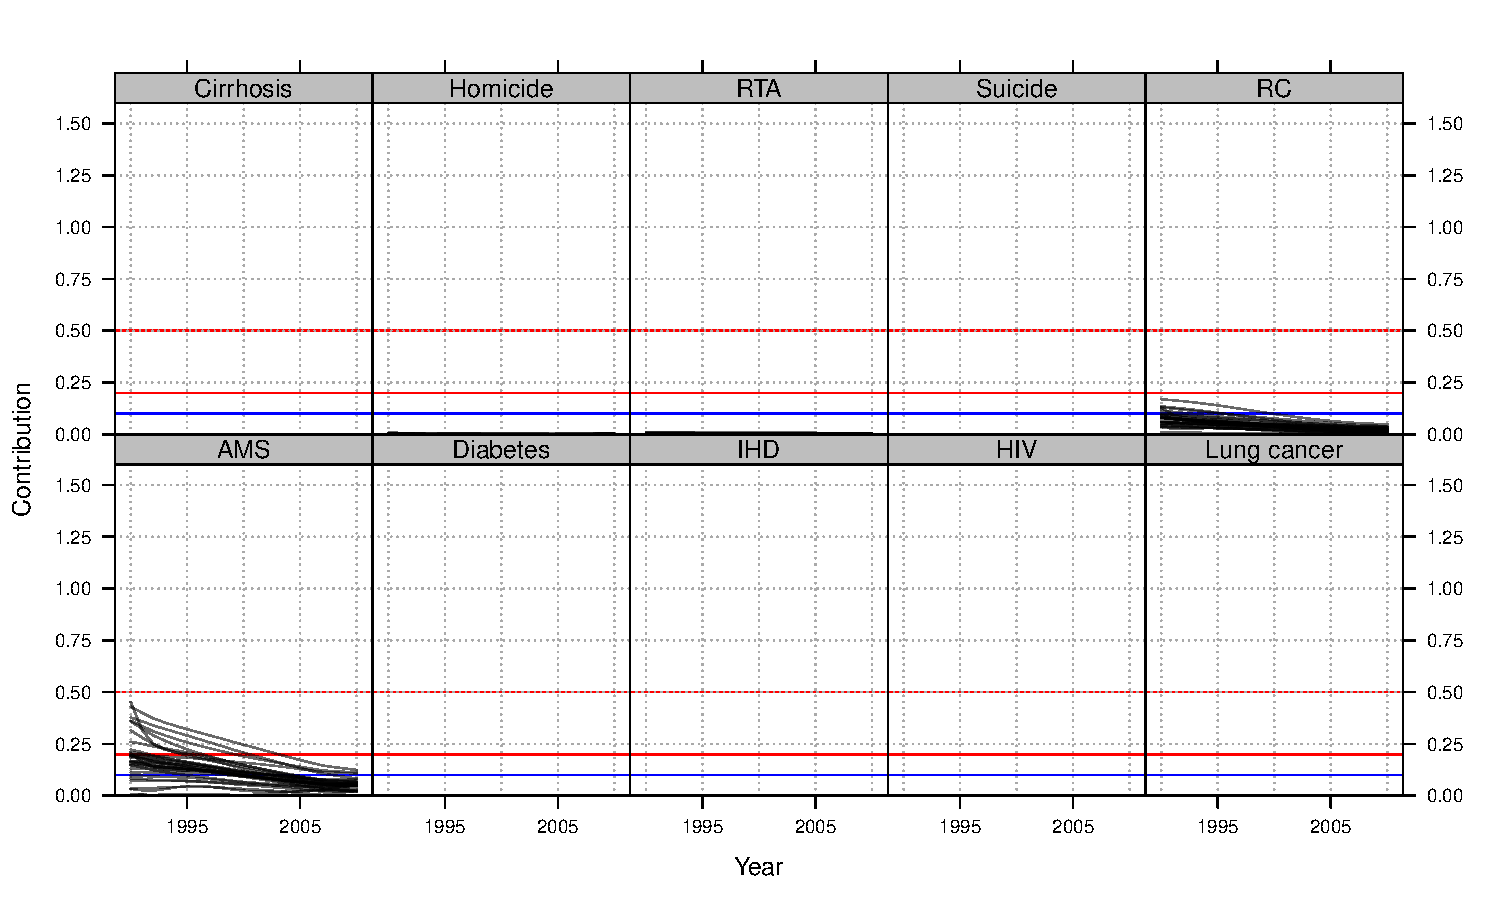
\includegraphics[scale=.5]{Figures/AM_0_14_females.pdf}
\end{subfigure}
Source: own calculations based on INEGI and SOMEDE files. 
\end{figure}




\begin{figure}
\label{fig:15_39_contributions}
\centering
\caption{Age and cause contributions to state differences from the best
practices trend for temporary life expectancy 15-39, 1990-2015.}
\begin{subfigure}{\textwidth}
\centering
\caption{Males}
\vspace{-2em}
\label{fig:e15_39_males}
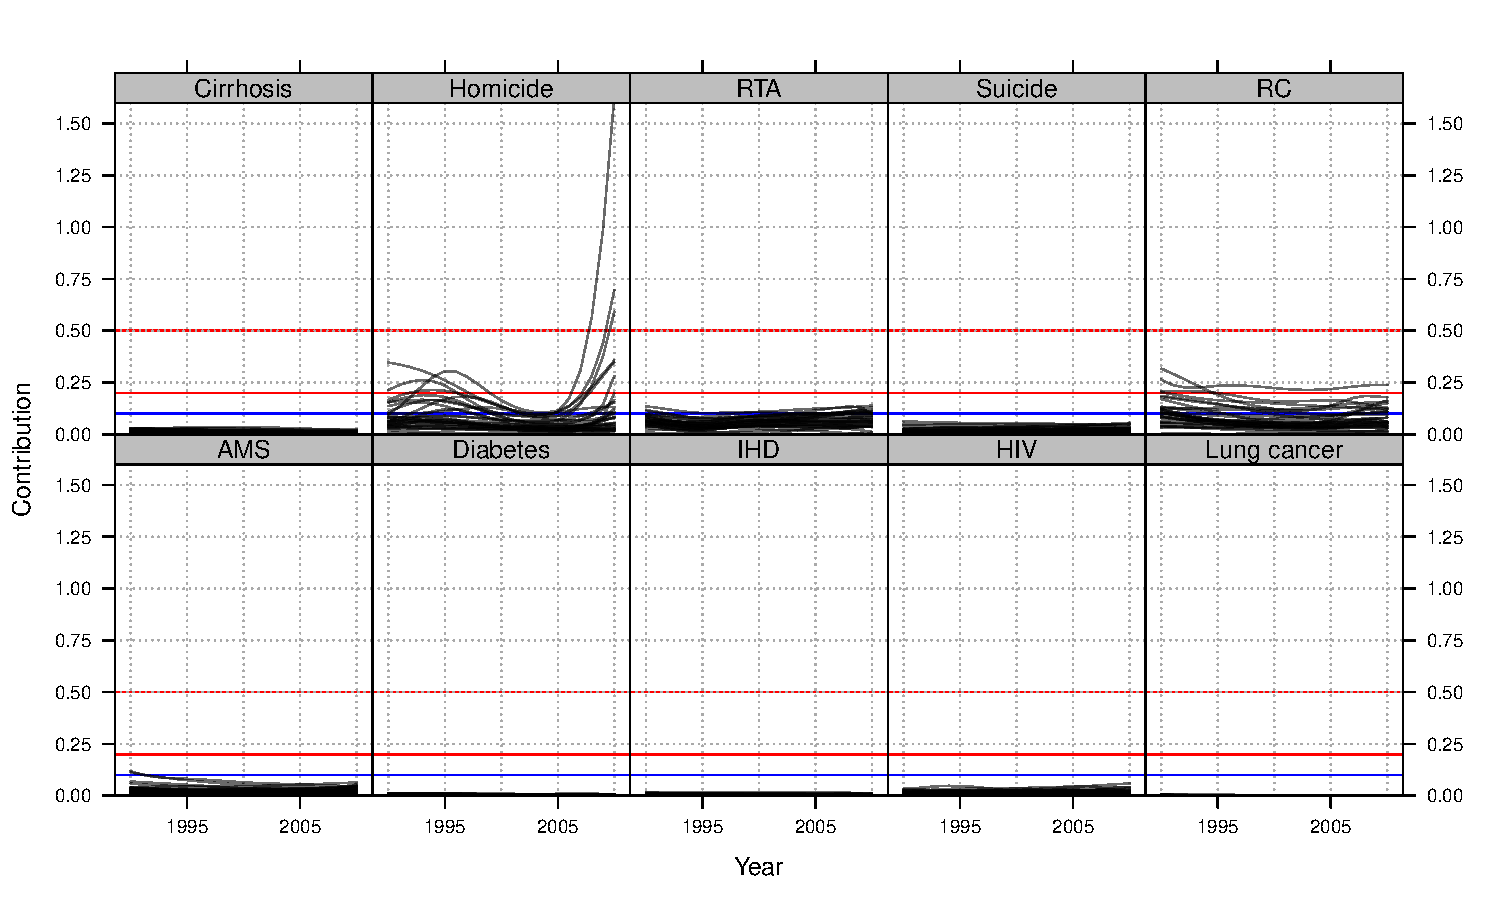
\includegraphics[scale=.5]{Figures/AM_15_39_males.pdf}
\end{subfigure}
\\
\begin{subfigure}{\textwidth}
\centering
\caption{Females}
\vspace{-2em}
\label{fig:15_39_females}
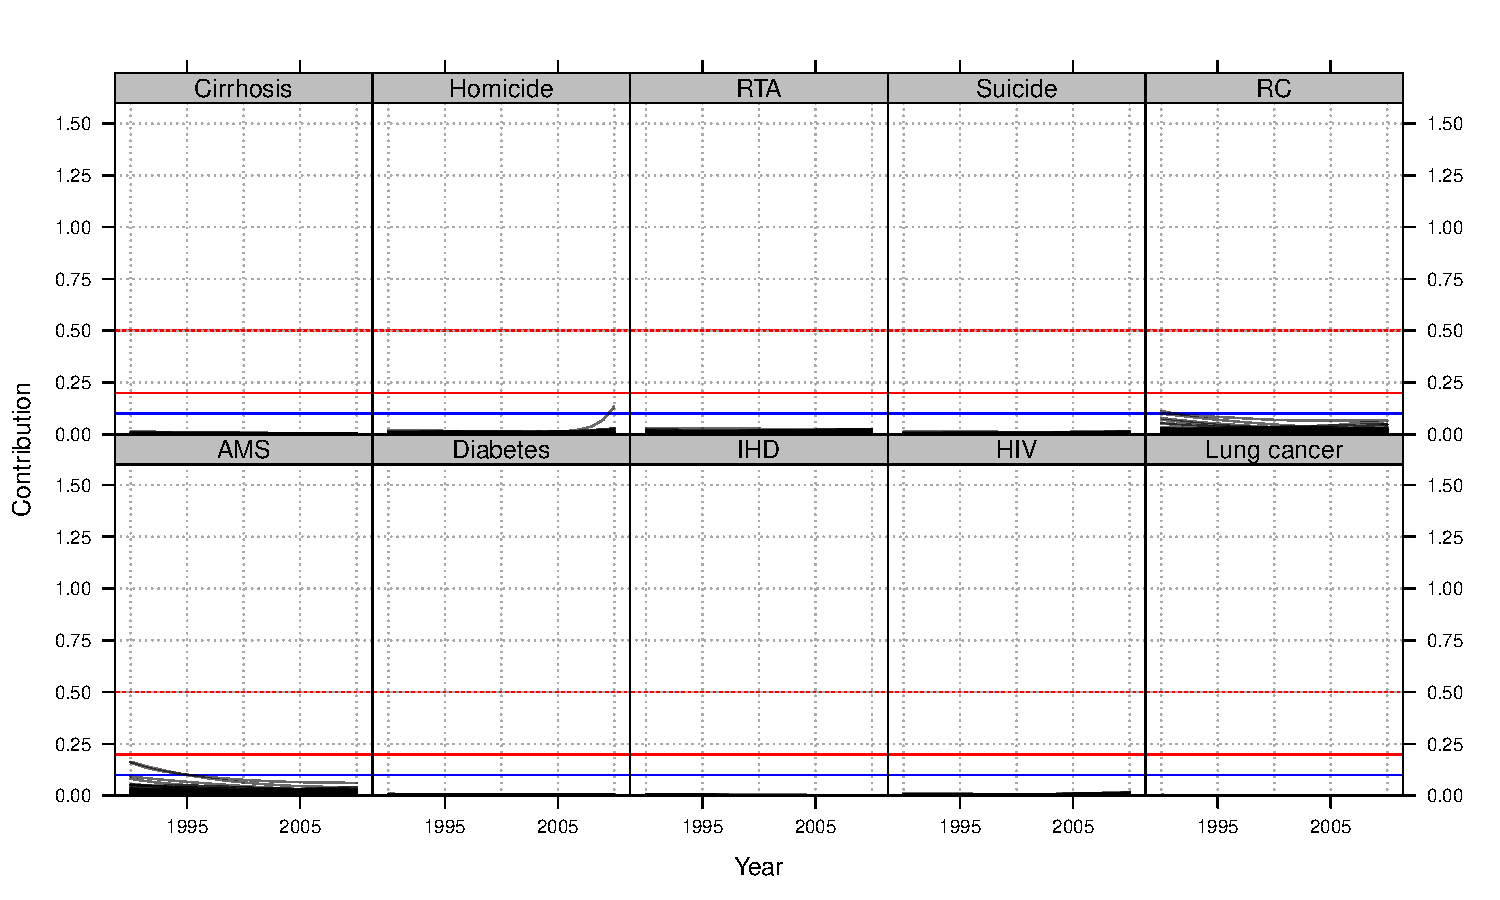
\includegraphics[scale=.5]{Figures/AM_15_39_females.pdf}
\end{subfigure}
Source: own calculations based on INEGI and SOMEDE files. 
\end{figure}


Adult mortality shows the largest deviations from the best practices life expectancy (Figure 4) in both males (\ref{fig:e40_74_males}) and females (\ref{fig:40_74_females}). Specifically, among men, conditions amenable to medical services, diabetes, IHD, cirrhosis and homicides have the largest toll on mortality, leading to the largest gap between the BP line and contributing to disparities among the states. For instance 12 of the 32 states are more than a quarter of life far from the best practices mortality, one of them with almost 0.75 years lagging behind. Similarly, diabetes and IHD show little improvements in the full period. Cirrhosis and homicide are at the heart of health deterioration among the adults. Both of them show large disparities within the states, ranging from values very close to zero in some states, to deviations over 1.25 years from the BP observed. After 2005, homicide shows an important increase in the gap from the minimum mortality observed. 

Results for women  (\ref{fig:40_74_females}) are different. Deviations from the BP line are mainly explained by the high mortality of conditions amenable to medical service, diabetes and IHD. These three categories show a steady pattern far from the BP mortality. On the contrary, Cirrhosis shows convergence to the minimum observed. The rest of conditions are very close to the BP line. 

\begin{figure}
\label{fig:40_74_contributions}
\centering
\caption{Age and cause contributions to state differences from the best
practices trend for temporary life expectancy 40-74, 1990-2015.}
\begin{subfigure}{\textwidth}
\centering
\caption{Males}
\vspace{-2em}
\label{fig:e40_74_males}
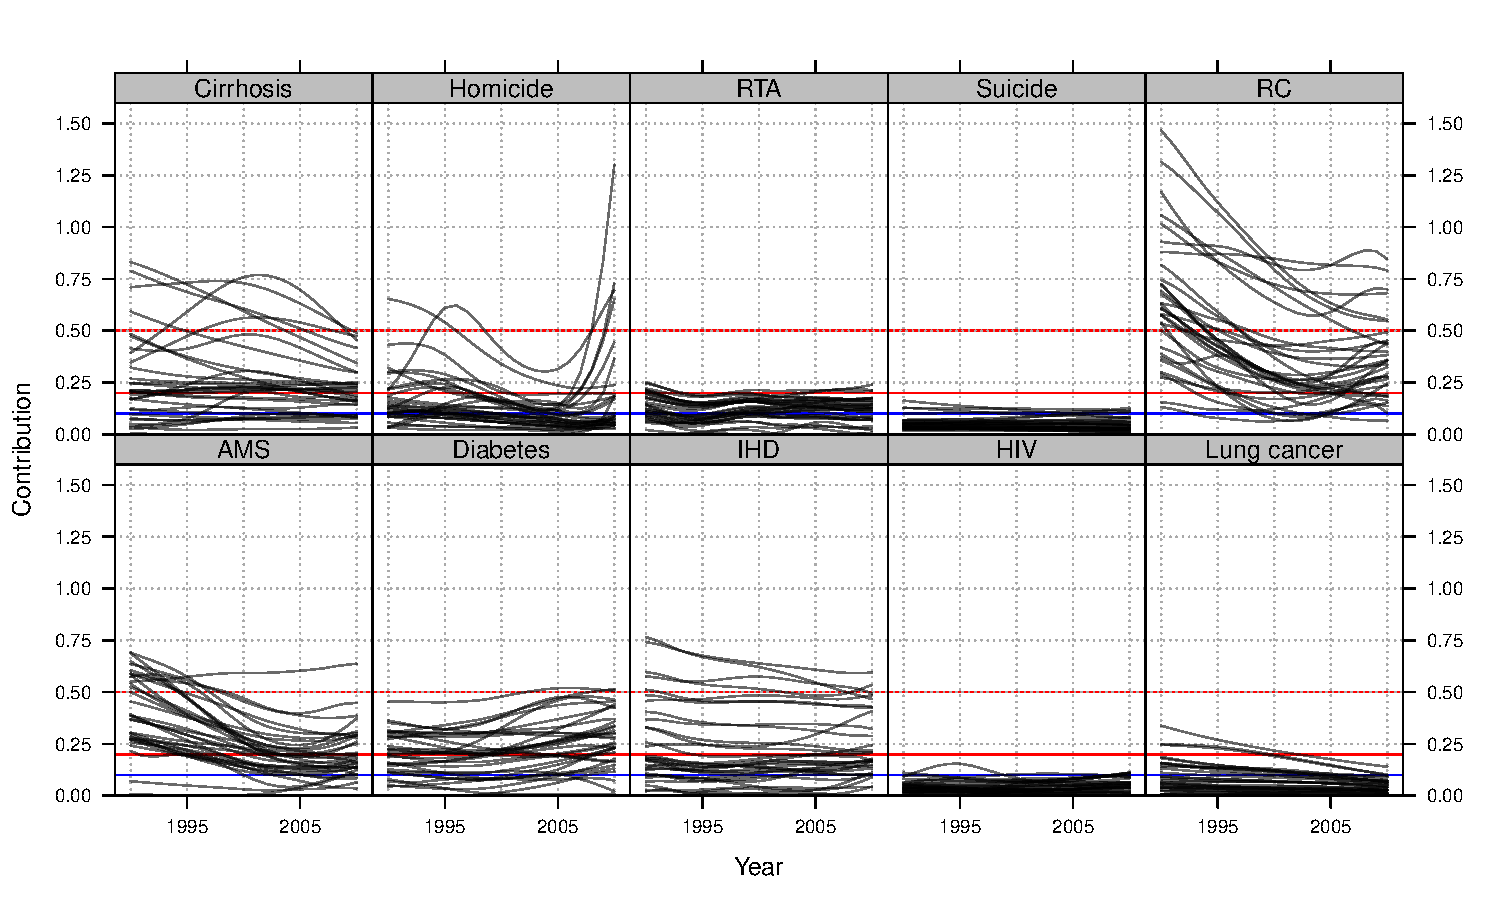
\includegraphics[scale=.5]{Figures/AM_40_74_males.pdf}
\end{subfigure}
\\
\begin{subfigure}{\textwidth}
\centering
\caption{Females}
\vspace{-2em}
\label{fig:40_74_females}
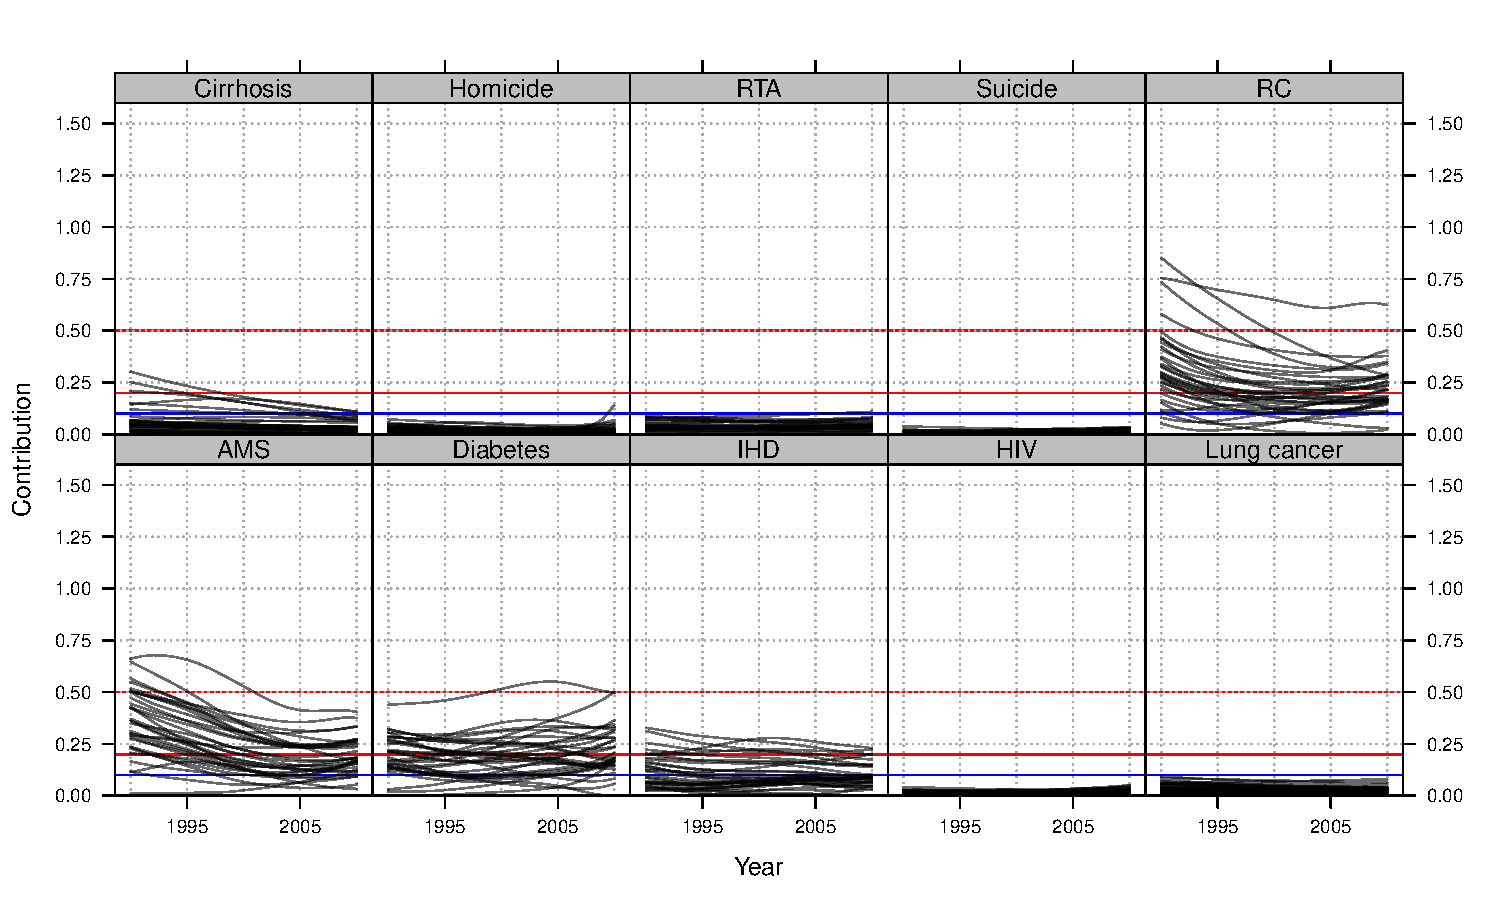
\includegraphics[scale=.5]{Figures/AM_40_74_females.pdf}
\end{subfigure}
Source: own calculations based on INEGI and SOMEDE files. 
\end{figure}



%\subsection*{Age and cause contributions to state differences from the best
%practices trend.}
%This section will be completed at a later date. Preliminary results are shown.
%\begin{figure}[h!]
%\caption{Cause-specific contributions to the difference between observed and BP. (preliminar figure)}
%\centering
%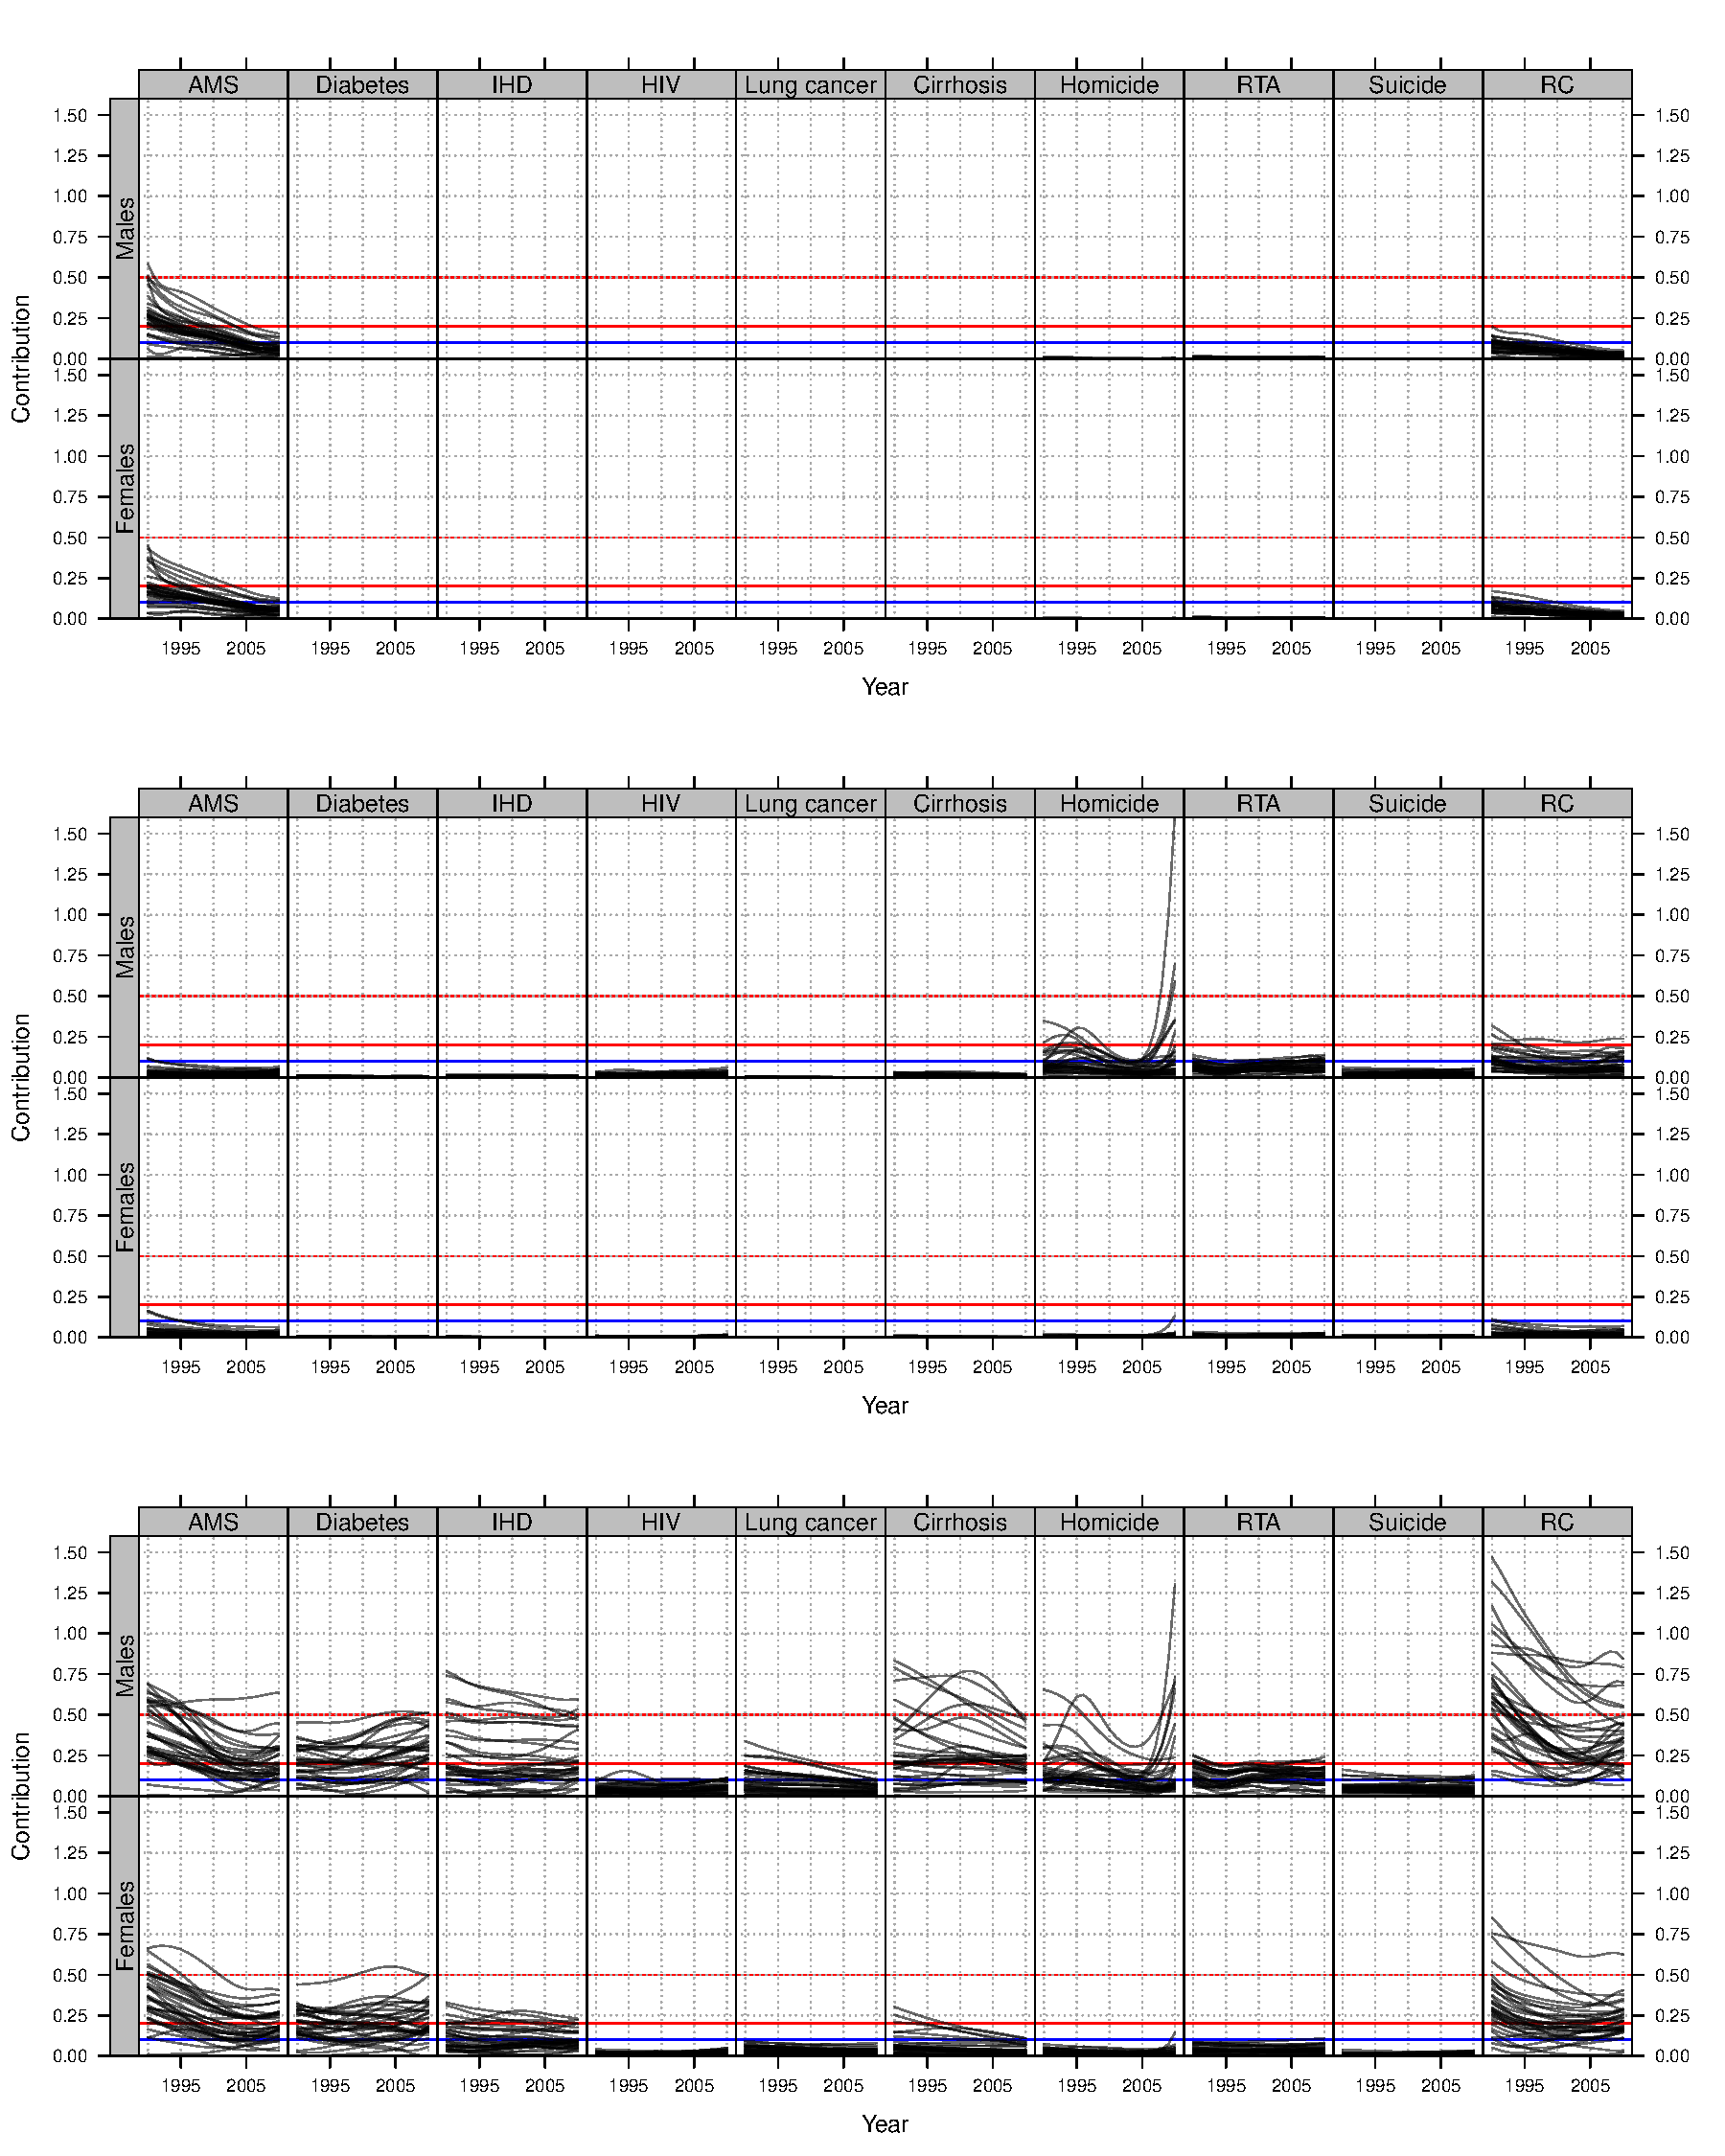
\includegraphics[scale=.4]{Figures/TLE_Decomp.pdf}
%Source: own calculations based on INEGI and SOMEDE
%\end{figure}


%This will show a few small multiples figures, tbd 

%\section*{Discussion}
%Talk about the role of homicide and other major causes. How many years of life
%were lost? (not just expectancy). maybe..

\section*{Discussion}
\subsection*{Trends in best practices life expectancy}
It is both curious and concerning that the best practices trends have not been
steadily increasing over the period studied. Rather, trends were irregular for
children, flat for adults, and decreasing for older adults. We expected
that the geographic diversity in Mexico would offset the recent mortality
setbacks known from states such as Chihuahua and Durango. If the best practices
trend determines our expectations for future mortality, we can conclude that
our expectations ought to have been stagnant or deflating over time, depending
on the age group considered. It would still represent a great success if
mortality were to drop to the best practices level in all states, as unrealistic as this may seem, but at the same time we expect
the best practices trend to increase given a mix of new technologies, reforms,
and improved material wellbeing.

\subsection*{Child and young-age mortality}
Despite this pessimistic finding about the best practices trend, all states have
converged toward the best practices temporary life expectancy for the age group
from 0 to 14 over the 21 years studied. Our results show that this has been due to improvements in causes amenable to medical service. Which is consistent with previous studies highlighting decreases in infectious and respiratory diseases in these ages \citep{canudas2014}. Moreover, major health care reforms and programs, such as Seguro Popular and Oportunidades (now Progresa) have focused efforts in reducing inequalities and improving health services for children. In fact, in 2012 78.3\% of children under age one visited a doctor to monitor their development and growth; however, children with social security showed a significantly greater effective access coverage  than those with Seguro Popular or no health insurance \citep{urquieta2015evolution}. Our results reinforce the success of such programs by bringing life expectancy up and narrowing the gap between the best practices trend and the state-specific life expectancy in these ages.

Males experienced the same positive trend of convergence in the age group 15 to
39 until the year 2006, when a sudden and sizeable excess in homicide mortality
began in particular states, especially on the Northern border with the U.S.A.
The surge in violent deaths overlapped with a more widespread and earlier
trend in increasing diabetes mortality. It is important to note that the
so-called accident hump grew manifold in size due to violent deaths in
particular states. Our results show that deviations from the best practices mortality in this age-group is mainly driven by the unprecedented rise in homicide mortality after 2005, which is consistent with previous research that highlight the burden of violence on population health between 2005-2010 \citep{Aburto2015}. We extended this previous analysis by adding information from 2011 to 2015. Our results show that the high prevalence of homicide mortality in these ages remain, which highlight the failure of the Mexican government to bring down the levels of violence that started rising after 2005. In fact, states like xxx are still experiencing high mortality rates provoking losses of life of xx years relative to the best practices mortality. Between-state variance in temporary life expectancy was much smaller for females over the same period, though females showed the same overall trend of convergence, followed by
divergence after 2006.

\subsection*{Old age mortality}
The main results of our study are the trends in older adult mortality.
For older adults in the 39 to 74 age group, all states except for Chihuahua and
Baja California converged, albeit not toward the best practices trend. Instead,
the best practices trend decreased toward the state trends. Males experienced no
notable improvements in these age groups over the period, while females only
experienced minor improvements, excepting Chihuahua and
Baja California. 

Improving health is a priority for governments of many developing countries, in part to achieve the Millennium Development Goals established for 2015.  Great improvements have been accomplished in reducing mortality and inequalities in children and the young population. Nevertheless, our results show that older adults are becoming a vulnerable group and more efforts are require to reduce the burden of conditions amenable to health services and policy/related conditions. In particular, this group lacks efforts on attending the burden of violence, through homicides; chronic-degenerative
causes of death, such as diabetes and isquemic heart diseases; and behavior-related conditions like homicide and cirrhosis. Of the three age groups considered, the older adult age group
has the most potential for gains in the future. All age groups considered have
room to improve, and many states have much potential for recovery.


After ten years of the implementation of the Popular Insurance program and more than 15 years after conditional transfers programs took place in Mexico, health disparities remain in the country with high, but achievable, challenges for the post-2015 agenda. As \citet{biosca2015} pointed out, these programs should also focus in the awareness of enrollment in health insurance programs to influence the population towards improving health behavior. Our results reinforce the need of such, among others public health interventions, with an special focus on older adults in the country. Nevertheless, the health component of the conditional transfers program Oportunidades targets women between 20 and 59 years old. We argue that such programs must be more inclusive and reach older population since, as we showed, a high number of years is being lost due to the lack of presence of effective and opportune health care service. 

In addition, previous research emphasized the need of public health interventions to lessen the burden of homicides on population's health observed in the first decade of the 21st century \citep{canudas2014, Aburto2015}. We extend the period five years and found that the toll of homicides on the population is still high and it is highly contributing to health inequalities in the young population, consistent with the previous trend observed \citep{canudas2014}. Moreover, our results underscore the impact of violence also in the older adult population reaching unprecedented levels after 2005 making the best practices trend decrease. 
\end{spacing}

\section*{Competing interest}
None to declare.

%However, they still remain the world's most unequal countries \citep{Barreto2012}.
%}
%\bibliographystyle{plainnat}
\newpage
 \bibliography{AburtoRiffe_Bib.bib}
 
 
 \newpage
\section*{Supplemental material}

Appendix Table 1. Definitions of cause-of-death categories using the \nth{9} and \nth{10} revision of the International Classification of Diseases.\\

{\renewcommand{\baselinestretch}{1}\selectfont

\begin{longtable}{p{8cm}p{4cm}p{4cm}ccc}
\hline
\textbf{Category} & \textbf{ICD-10} & \textbf{ICD-9}\\
\hline
\endfirsthead
\multicolumn{3}{c}%
{\tablename\ \thetable\ -- \textit{Continue}} \\
\hline
\textbf{Category} & \textbf{ICD-10} & \textbf{ICD-9}\\
\hline
\endhead
\hline \multicolumn{3}{r}{\textit{Continues}} \\
\endfoot
\hline
\endlastfoot
\multicolumn{3}{l}{\bf I. Amenable to medical service}  \\
 I.A. AM-Infectious \& respiratory diseases : intestinal infections, tuberculosis, zoonotic bacterial diseases, other bacterial diseases, septicemia, poliomyelitis, measles, rubella, infectious hepatitis, ornithosis, rickettsioses/ arthropod-borne, syphilis (all forms), yaws, respiratory diseases, influenza \& pneumonia, chronic lower respiratory diseases & A00-A09, A16-A19, B90, A20-A26, A28, A32, A33, A35, A36, A37, A40-A41, A80, B05-B06, B15-B19, A70, A68, A75, A77, A50-A64, A66, J00-J08, J20-J39, J60-J99, J09-J18, J40-J47 & 001-009, 010-018, 32, 33, 37, 137, 020-027, 38, 45, 55-56, 70, 73, 080-082, 087, 090-099, 102, 460-479, 500-519, 480-488, 490-496 \\
           I.B. AM-Cancers: malignant neoplasm of colon, skin, breast, cervix, prostate, testis, bladder, kidney-Wilm's tumor only, eye, thyroid carcinoma, Hodgkin’s disease, leukemia & C16,C18-C21, C43-C44, C50, C53, C61, C62, C67, C64, C69, C73, C81, C91-C95 & 153-154, 172-173, 174, 180, 185, 186, 188-189, 190, 193, 201, 204-208\\
           I.C. AM-Circulatory: active/acute rheumatic fever, chronic rheumatic heart disease, hypertensive disease, cerebrovascular disease & I00-I02, I05-I09, I10-I13, I15, I60-I69 & 390-392, 393-398, 401-405, 430-438\\
          I.D. AM-Birth: maternal deaths (all), congenital cardiovascular anomalies, perinatal deaths (excluding stillbirths) & O00-O99, Q20-Q28, P00-P96 & 630-676, 745-747, 760-779\\
          I.E. AM-Other: disease of thyroid, epilepsy, peptic ulcer, appendicitis, abdominal hernia, cholelithiasis \& cholecystitis, nephritis, benign prostatic hyperplasia, misadventures to patients during surgical or medical care, cisticerchosis & E00-E07, 40-G41, K25-K27, K35-K38, K40-K46, K80-K81,  N00-N07, N17-N19, N25-N27, N40, Y60-Y69, Y83-Y84, B69 & 240-246, 345, 531-533, 540-543, 550-553, 574-575.1, 580-589, 600, E870-E876, E878-E879\\
 & \\          
 {\bf II. Diabetes}  & E10-E14 & 250 \\      
 & \\
 {\bf III. Ischemic Heart Diseases (IHD)}   & I20-I25 & 410-414, 429.2\\
 & \\           
 {\bf IV. HIV/AIDS} & B20-B24 & 279.1, 042-044\\ 
  & \\                
{\bf V. Lung cancer}  & C33-C34 & 162\\
  & \\          
{\bf VI. Cirrhosis}&  K70 & 571.1-571.3\\
 & \\          
{\bf VII. Homicides}  & X85-Y09 & E960-E969\\     
 & \\           
 {\bf VIII. Road traffic accidents}  & V01-V99 & E810-E819 \\     
 & \\           
{\bf IX. Suicide and self-inflicted injuries}  & U03, X60-X84, Y87.0 & E950-E959\\ 
 & \\          
{\bf X. Residual Causes }:  other cancers and other heart diseases & C00-D48, I00-I99 if not listed above, R00-R99 & 140-239, 390-459 if not listed above, 780-799
\label{ME_Mex}
\end{longtable}
}


\end{document}



